\chapter{Power Analysis}
\label{poweranalysis}
Power analysis utilizes the fact that different operations have different power consumptions.
By capturing the power consumption traces (power traces in short) and examining them, an attacker can reason about the variables determining the control flow during program execution.
If these variables are cryptographic secrets, or keys (e.g. private keys in RSA), they are leaked to the attacker in what is called a simple power analysis (SPA) attack\cite{kocher1999differential}.
In many cases the control is not related to the key, requiring more complex attacks.
For these cases capturing a large number of traces and performing statistical analysis can leak information about \emph{individual values}.
The two main attacks of this type are called differential power analysis (DPA)\cite{kocher1999differential} and correlation power analysis (CPA)\cite{brier2004correlation}.
All variants and the setup required are explained in this section.

\section{Setup}
Performing \poweranalysis{} requires access to the device in a controlled environment.
The attacker needs to control the power supply for the target, and be able to alter the containing electronics.
This is fairly easy for embedded platforms, as they are often made to be self-contained.
Even for more complex targets like IoT devices, the processor can be removed from its circuit board and put in an attack environment\cite{ronen2017iot}.

The setup for a \poweranalysis{} attack is as follows:
An attacker solders a resistor between the target processor and the ground connector of its power supply.
She then measures the voltage difference between both ends of the resistor with an oscilloscope.
This voltage is directly proportional to the current flowing through the resistor, and thus to the power consumption of the target.
The voltage recordings from the oscilloscope are then transferred to a computer, and can be analyzed there.

\section{Simple Power Analysis}
In the simplest form of \poweranalysis{}, SPA, power traces are usually examined visually.
Repeating patterns of operations can often be identified, leaking information about the control flow.
If the control flow is dependent on a key, an attacker can infer its value.
An example target would be RSA decryption being calculated via the square-and-multiply algorithm.
The difference between the multiply and the square operation is directly observable from power traces.
As the order of these operations is linked to the private key, identifying the control flow leaks the private key.
\Cref{fig:spa} shows a trace for square-and-multiply in RSA decryption, including the leaked private key bits.

\begin{figure}[h]
  \centering
  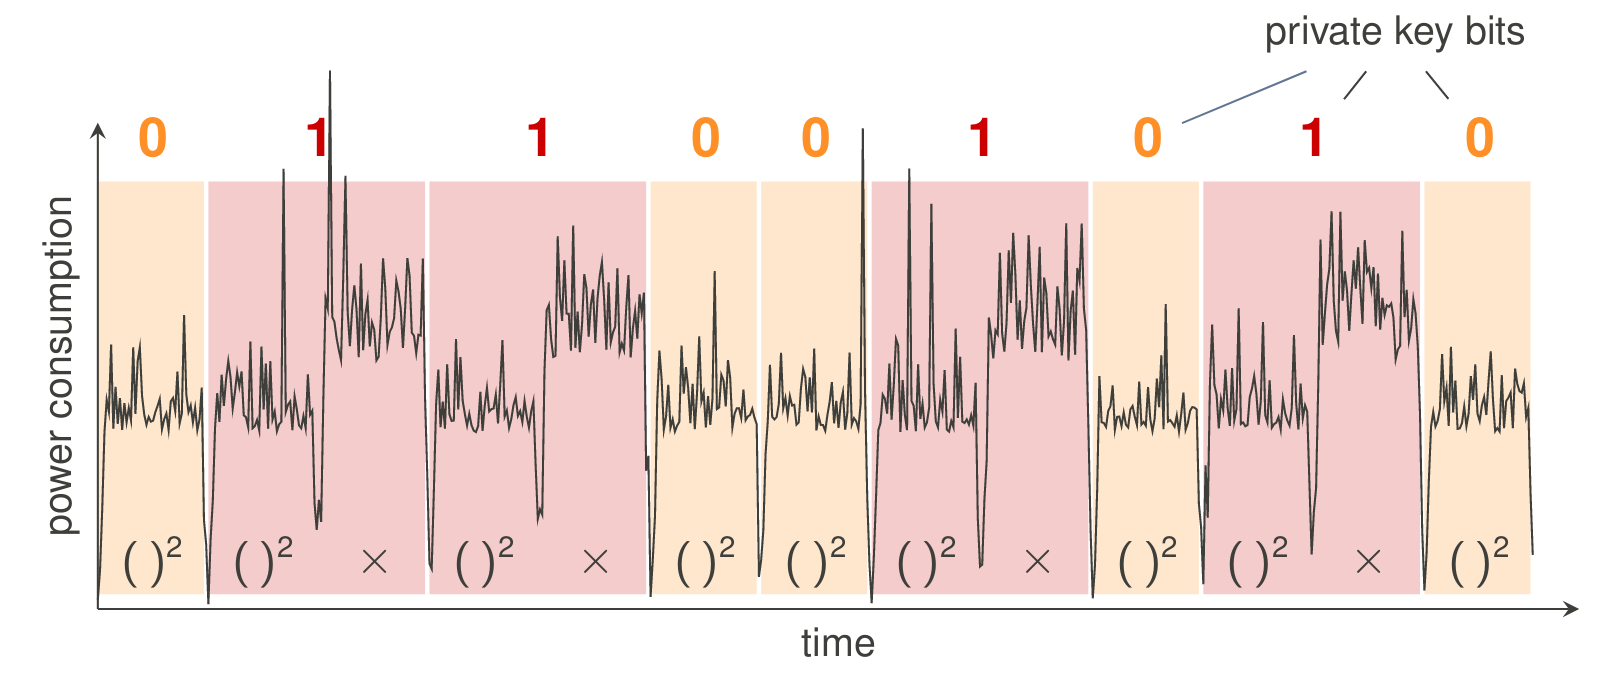
\includegraphics[width=\textwidth]{spa.png}
  \caption{Simple power analysis on square-and-multiply RSA\cite{boehme2017netsec}}
  \label{fig:spa}
\end{figure}

Power traces are often not as clear as in \Cref{fig:spa}, and contain some amount of random noise.
By averaging multiple traces this noise can be reduced, allowing for easier analysis.

\section{Differential Power Analysis}
The control flow is often not enough to leak the entire key, and it is very hard to gain information about the actual data from only SPA.
For this a more complex variant of \poweranalysis{} can be used, namely \emph{Differential \poweranalysis{}} (DPA).
DPA requires a large number of power traces, with the cryptographic algorithm being run on a known plaintext in each execution.
It also requires that the attacker knows which cryptographic algorithm is running on the target.
Both of these requirements are usually fulfilled in embedded devices.

The attacker additionally requires a \emph{power model}, which is used to calculate the expected power consumption for a given value.
While not entirely accurate\cite{brier2004correlation}, the \hammingw{} has proven to be a very effective power model in practice.

Knowing the algorithm running on the target, the attacker can predict the result of intermediate computations, given some assumption about the key.
In practice she usually guesses a single key bit, and then calculates the expected result of some bitwise operation, e.g. XOR.
The other bits are not important for her attack at the moment and are thus ignored.
After calculating the expected power consumption for all plaintexts, she splits the power traces in two subsets, based on the value of the expected result.
Then she calculates the mean of both sets, and calculates their difference.
If the guess for the current key bit was correct, then all traces in a single subset will have the same value for the current bit.
This means that the difference between both means shows spikes in the places where the attacked operation happens.

If the guess was wrong on the other hand, the values of the current bit are randomly distributed in both sets, and the difference will show no spikes of non-zero values.
The values of the other bits can be ignored, as they are close enough to being random in both sets, and thus filtered out by calculating the difference.
Other power consumption noise, coming from different parts of the processor, is randomly distributed overy every trace, and thus filtered by taking the mean.
Both the values for other bits and other power consumption influences are note entirely random, but close enough to it that these assumptions work well in practice.

\Cref{fig:dpa} shows a typical DPA result with the mean power consumptions of both sets, the difference between the two, and the difference with the Y axis magnified by a factor of 15.
This analysis was performed on the output of the least significant bit after the first S-box substitution in AES.
\begin{figure}[h]
  \centering
  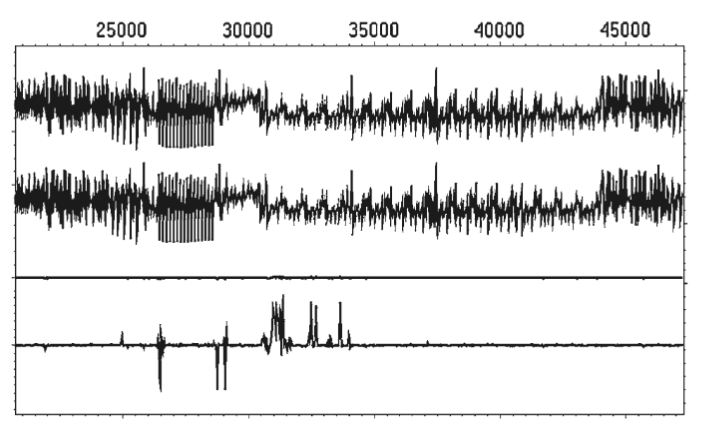
\includegraphics[width=0.8\textwidth]{dpa.png}
  \caption{Difference in means during DPA\cite{kocher2011introduction}}
  \label{fig:dpa}
\end{figure}

\section{Correlation Power Analysis}
CPA is the most complex of these attacks, but also offers the best results.
The attacker starts by making a list of candidate values for a part of the key, usually individual bytes.
With a power model, usually the \hammingw{} like for DPA, she can calculate the expected power consumption for combination of key guess with every plaintext.

For a fixed key guess, these expected power consumptions are a function over all plaintexts.
For a single point in time, the actual power traces are \emph{also} a function over all plaintexts, with the actual key being a fixed parameter unknown to the attacker.
By testing how much the expected power consumptions correlate with the actual power consumptions, the attacker can find the confidence values of the guesses for the current part of the key.
She then assumes the value with the highest correlation coefficient is correct, and continues her attack for the rest of the key.

Of course the attacker does not know exactly which point in time she is supposed to examine.
However, it is very unlikely that an incorrect key guess at a random point in time has a closer correlation than the correct key guess at the correct time, and so an attacker can simply use the maximum correlation coefficient.

\section{Defenses Against Power Analysis Attacks}
Defenses against this class of attack usually work by either adding additional factors to the power consumption, thus increasing the computational effort required for analysis, or by reducing variances in power consumption altogether.
This reduced variance decreases the information an attacker can gain from the same number of power traces, giving her reduced confidence in her result or requiring her to capture more traces.

Masking\cite{golic2002multiplicative}\cite{coron2000boolean} for example is an algorithm specific defensive measure that adds a third factor to the power consumption by first performing adding a masking value to the plaintext via an invertible operation.
The cryptographic algorithm then works on the masked value, and only in the end unmasks the result.
As such the attacker has to calculate her correlation for each possible combination of key byte and mask value.
This increases the number of traces she needs to capture (to still provide the same confidence in her analysis) and the computation time of her analysis.

Other defensive measures focus on creating a worse signal to noise ratio for the entire power consumption.
One technique that has gained a lot of traction is \dual{}\cite{sokolov2005design}.
It works by calculating the inverse of every intermediate result along with the actual result, thus balancing the number of 1s.
This results in a constant \hammingw{} and therefore a data-independent power consumption.

Unfortunately, \dual{} suffers from multiple engineering problems.
The power required to set the value of a bit to 1 is dependent on properties of the underlying transistors, which are subject to variances in manufacturing.\cite{razafindraibe2006formal}
Minimal differences in clock timings between both paths can also reduce the security of \dual{}\cite{baddam2008path}.
Storing the inverse also requires significantly larger circuitry, doubling the circuit size or more\cite{baddam2008path}.

Even with these caveats, \dual{} has the major advantage that once it is applied, \emph{any} code can be run without modifications while still benefiting from the increased robustness.
